\section{1174095 - Muhammad Dzihan Al-Banna}
\subsection{Teori}
\begin{enumerate}

	\item Jelaskan apa itu klasifikasi teks, sertakan gambar ilustrasi buatan sendiri.
	\hfill\break
	Klasifikasi teks merupakan sebuah model yang biasa digunakan untuk untuk mengkategorikan sebuah teks ke dalam kelompok-kelompok yang lebih terorganisir. Jadi untuk setiap kalimat yang di masukan ke dalam mesin, mesin tersebut akan menjadikan setiap kata dari kalimat tersebut menjadi sebuah kolom. Untuk ilustrasinya bisa dilihat pada gambar berikut : 

	\begin{figure}[H]
	\centering
		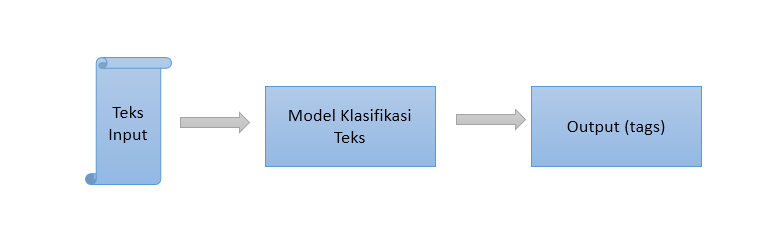
\includegraphics[width=4cm]{figures/1174095/tugas4/1.PNG}
		\caption{Klasifikasi teks.}
	\end{figure}

	\item Jelaskan mengapa hal ini bisa terjadi, klasifikasi bunga tidak bisa digunakan untuk machine learning, sertakan ilustrasi gambar sendiri.
	\hfill\break
	Karena machine learning tidak dapat menampilkan inputan sesuai dengan apa yang kita inputkan. Karena inputan tersebut serupa namun mesin memberikan output yang berbeda, biasanya output atau error ini disebut dengan istilah noise. Untuk contoh sederhananya misalkan kita inputkan salah satu label yang terdapat pada bunga, output yang dihasilkan oleh mesin tersebut ialah label yang lain. Itu dikarenakan bunga banyak jenis yang serupa namun tidak sama. Untuk ilustrasinya bisa dilihat pada gambar berikut : 

	\begin{figure}[H]
	\centering
		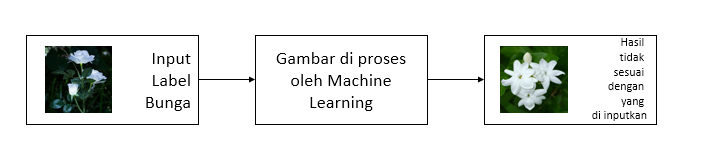
\includegraphics[width=4cm]{figures/1174095/tugas4/2.PNG}
		\caption{Klasifikasi Bunga.}
	\end{figure}
	
	\item Jelaskan bagaimana yang dimaksud dengan teknik pembelajaran mesin pada teks yang digunakan dan sertakan ilustrasi buatan sendiri.
	\hfill\break
	Teknik yang digunakan pada youtube salah satunya ialah keywords. Dengan keywords tersebut mesin dapat memberikan video sesuai dengan keyword yang kita inputkan pada kolom pencarian. Teknik pembelajarannya tergantung user memberikan input teks seperti apa, karena pada youtube itu sendiri akan menyesuaikan dengan apa yang biasa kita inputkan dan akan memfilter video secara otomatis sesuai dengan keyword yang biasa kita inputkan. Contoh ilustrasi sederhananya seperti berikut :

	\begin{figure}[H]
	\centering
		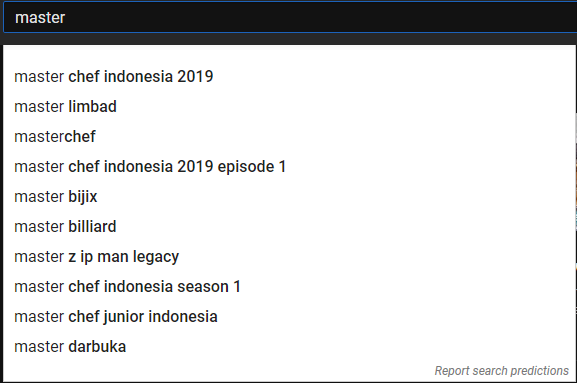
\includegraphics[width=4cm]{figures/1174095/tugas4/3.PNG}
		\caption{Klasifikasi teks Youtube.}
	\end{figure}

	\item Jelaskan apa yang dimaksud vektorisasi data.
	\hfill\break
	Vektorisasi data ialah suatu pemecahan atau pembagian data berupa teks, sebagai contoh terdapat 5 paragraf, data teks tersebut di pecah menjadi kalimat-kalimat yang lebih sederhana, lalu di pecah lagi menjadi kata untuk setiap kalimatnya. 

	\item Jelaskan apa yang dimaksud dengan bag of words dengan ilustrasi sendiri.
	\hfill\break
	Representasi penyederhanaan sebuah kalimat atau perhitungan setiap kata pada suatu kalimat dengan presentase berapa kali muncul kata tersebut untuk setiap kalimatnya. Contoh ilustrasi sederhananya seperti berikut : 

	\begin{figure}[H]
	\centering
		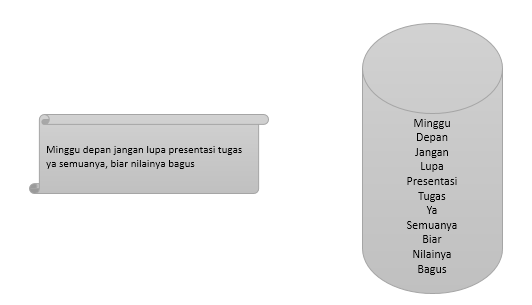
\includegraphics[width=4cm]{figures/1174095/tugas4/4.PNG}
		\caption{Decision Tree.}
	\end{figure}

	\item Jelaskan apa yang dimaksud dengan TF-IDF.
	\hfill\break
	TF-IDF merupakan metode untuk menghitung bobot setiap kata pada suatu kalimat yang paling sering digunakan. TF-IDF ini akan menghitung nilai Term Frequency dan Inverse Document Frequency pada setiap kata dalam setiap kalimat yang muncul dengan diimbangi dengan jumlah dokumen dalam korpus yang mengandung kata. Contoh ilustrasi sederhananya seperti gambar berikut : 

	\begin{figure}[H]
	\centering
		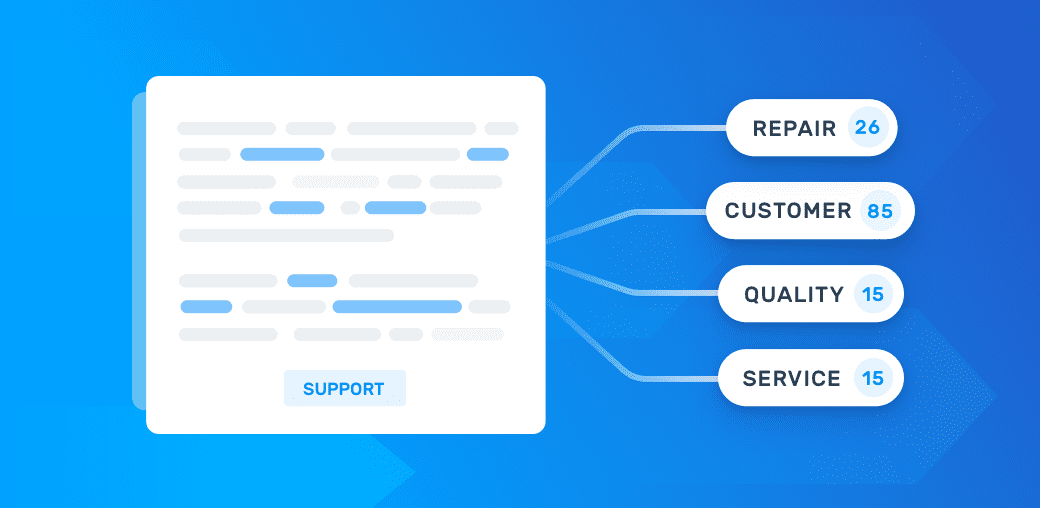
\includegraphics[width=4cm]{figures/1174095/tugas4/5.PNG}
		\caption{TF-IDF.}
	\end{figure}
\end{enumerate}

    \subsection{Praktek}
    \begin{enumerate}
        \item import data pandas dan 500 baris data dumy kemudian di jelaskan tiap barisnya. \hfill \break \lstinputlisting[firstline=8, lastline=12]{src/1174095/tugas4/praktek1.py}
        
        \begin{figure}[H]
            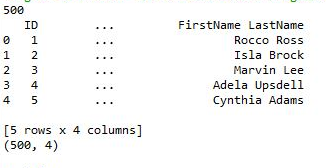
\includegraphics[width=4cm]{figures/1174095/tugas4/h1.PNG}
            \centering
            \caption{Data Dummy}
        \end{figure}

        \item memecah data prame menjadi dua yag pertama 450 dan kedua sisanya \hfill \break \lstinputlisting[firstline=13, lastline=21]{src/1174095/tugas4/praktek2.py}
        
        \begin{figure}[H]
            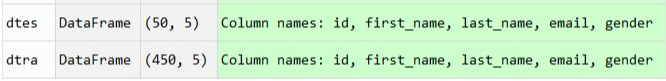
\includegraphics[width=4cm]{figures/1174095/tugas4/h2.PNG}
            \centering
            \caption{Pisah Data}
        \end{figure}

        \item praktek vektorisasi \hfill \break \lstinputlisting[firstline=12, lastline=49]{src/1174095/tugas4/praktek2.py}
        
        lakukan import library pandas yang di inisialisasi menjasi pd setelah itu ada dibuat variable data dengan method read\_csv untuk membaca file berekstensikan csv yang di masukan alamatnya pada kurung, lakukan klasifikasi atau pemilihan komentar yang berisi spam atau bukan spam dengan parameter class samadengan 1 merupakan spam dan class samadengan 0 bukan spam setelah itu masukan librari CountVektorizer yang digunakan untuk vektorisasi data kemudian dilanjutkan pada bagian In[103] dibuat variabel yang berisi vektorisasi dari data pada data di field content setelah itu variabel tersebut di running hasilnya menunjukan 350 baris di kali 1738 kolom selanjutnya dicoba untuk memunculkan isi recod pada baris ke 345 maka akan muncul isian dari baris tersebut. selanjutnya dibuat variabel dk atau daftar yang berisi data hasil vektorisasi setelah yang terdiri dari variabel dshuf yang berisi data komen yang di dalamnya di buat random yang nantinya akan dibut data training dan data testing dengan ketentuan data training 300 dan data testing sebanyak 50 setelah itu data training di lakukan vektorisasi dan data testing juga dilakukan vektorisasi setelah itu kedua data training dan testing tersebut dibuat label dengan parameter field CLASS pada tabel.
        \begin{figure}[H]
            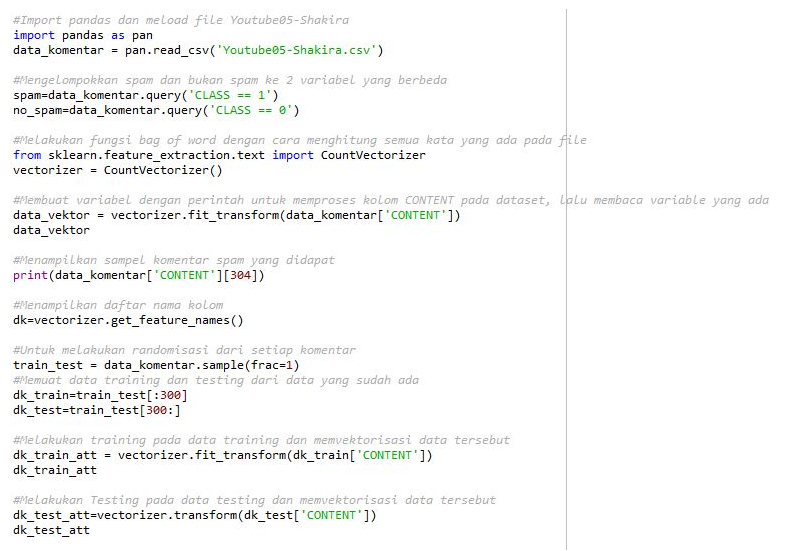
\includegraphics[width=4cm]{figures/1174095/tugas4/h3.PNG}
            \centering
            \caption{Vektorisasi}
        \end{figure}

        \item klasifikasi SVM \hfill \break \lstinputlisting[firstline=53, lastline=56]{src/1174095/tugas4/praktek2.py}
        
        import librari svm dari sklearn kemudian membuat variabel clfsvm berisikan method svc setelah itu variabel tersebut di berikan method fit dengan isian data train vektorisasi dan data training label yang berguna untuk melatih data tersebut setelah itu di coba untuk memunculkan score atau akurasi dari data tersebut menggunakan data testing vektorisasi dan data testing label.
        \begin{figure}[H]
            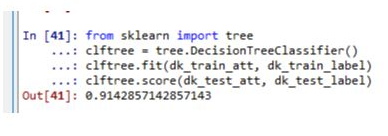
\includegraphics[width=4cm]{figures/1174095/tugas4/h4.PNG}
            \centering
            \caption{SVM}
        \end{figure}

        \item klasifikasi decision tree \hfill \break \lstinputlisting[firstline=61, lastline=65]{src/1174095/tugas4/praktek2.py}
        
        import librari tree dari sklearn kemudian membuat variabel clftree berisikan method DecisionTreeClasifier setelah itu variabel tersebut di berikan method fit dengan isian data train vektorisasi dan data training label yang berguna untuk melatih data tersebut agar dapat digunakan pada codingan selanjutnya setelah itu di coba untuk memunculkan score atau akurasi dari data tersebut menggunakan data testing vektorisasi dan data testing label.
        \begin{figure}[H]
            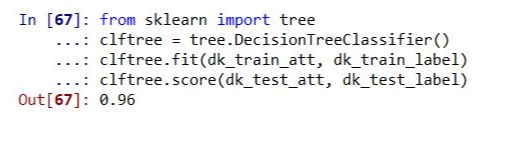
\includegraphics[width=4cm]{figures/1174095/tugas4/h5.PNG}
            \centering
            \caption{Desicion Tree}
        \end{figure}

        \item plot comfusion matrix \hfill \break \lstinputlisting[firstline=68, lastline=71]{src/1174095/tugas4/praktek2.py}
        
        import library comfusion matrix selanjutnya dilakukan prediksi pada pada data tes nya kemudian data tersebut di masukan kedalam variabel cm dengan method confusion matrix yang di dalamnya terdapat data dari variabel perd label dan dk test label setelah itu variabel cm tersebut di running maka akan memunculkan nilai matrixnya. 
        \begin{figure}[H]
            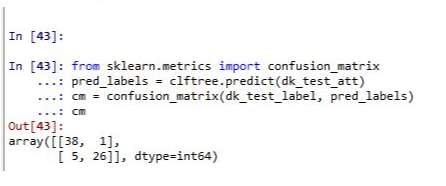
\includegraphics[width=4cm]{figures/1174095/tugas4/h6.PNG}
            \centering
            \caption{Confussion Matrix}
        \end{figure}

        \item cross valodation \hfill \break \lstinputlisting[firstline=74, lastline=89]{src/1174095/tugas4/praktek2.py}
        
        memunculkan nilai akurasi dari tiga metode yaitu random forest, decision tree, dan klasifikasi svm (suport vector machine) diamana akan di bandingkan tingkat akurasi dari semua hasil akurasiya mana yang terbaik dan lebih akurat pada hasilnya data yang paling akurat yaitu random forest.
        \begin{figure}[H]
            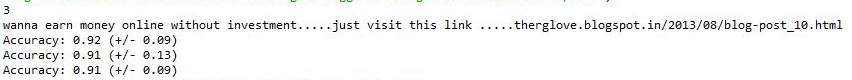
\includegraphics[width=4cm]{figures/1174095/tugas4/h7.PNG}
            \centering
            \caption{Cross Validation}
        \end{figure}

        \item Pengamatan program \hfill \break \lstinputlisting[firstline=92, lastline=106]{src/1174095/tugas4/praktek2.py}
        
        terdapat grafik data yang terdapat dari grafik tersebut di dapat dari codingan dengan cara pengulangan data masing masing 10 kali setelah itu di eksekusi menjadi grafik berbentuk 3D pada gambar tersebut menunjukan rasio dari yang terrendah yaitu data SVM kemudian data decision tree dan hasil random forest.
        \begin{figure}[H]
            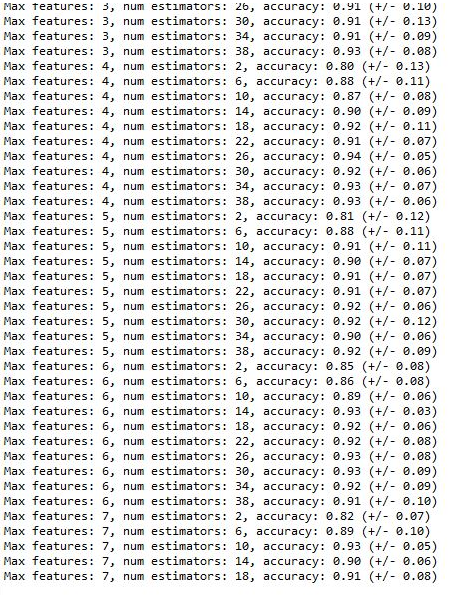
\includegraphics[width=4cm]{figures/1174095/tugas4/h8.PNG}
            \centering
            \caption{Pengamatan Program}
        \end{figure}

        Berikut adalah untuk grafik \hfill \break \lstinputlisting[firstline=110, lastline=124]{src/1174095/tugas4/praktek2.py}
        \begin{figure}[H]
            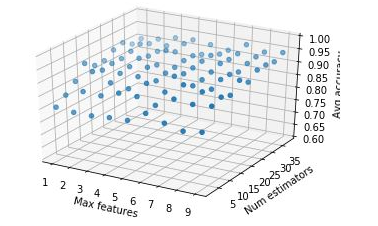
\includegraphics[width=4cm]{figures/1174095/tugas4/h9.PNG}
            \centering
            \caption{Grafik}
        \end{figure}
    \end{enumerate}
    \subsection{Penanganan Error}
        \subsubsection{Sreenshoot Error}
        \begin{enumerate}
            \item Error 1
            \begin{figure}[H]
                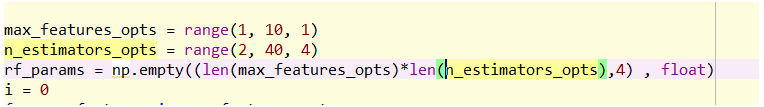
\includegraphics[width=4cm]{figures/1174095/tugas4/err1.PNG}
                \centering
                \caption{Error1}
            \end{figure}
        \end{enumerate}
        \subsubsection{Kode Error dan Jenisnya}
        \begin{enumerate}
            \item Kode Error 1 jenis Name Error
            \begin{figure}[H]
                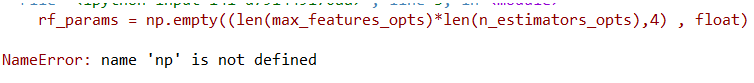
\includegraphics[width=4cm]{figures/1174095/tugas4/err2.PNG}
                \centering
                \caption{Error1}
            \end{figure}
        \end{enumerate}
        \subsubsection{Solusi}
        \begin{enumerate}
            \item 
            Solusi dari error di atas adalah dengan cara mengimport numpy as np
        \end{enumerate}

\subsection{Bukti Tidak Plagiat}
\begin{figure}[H]
\centering
	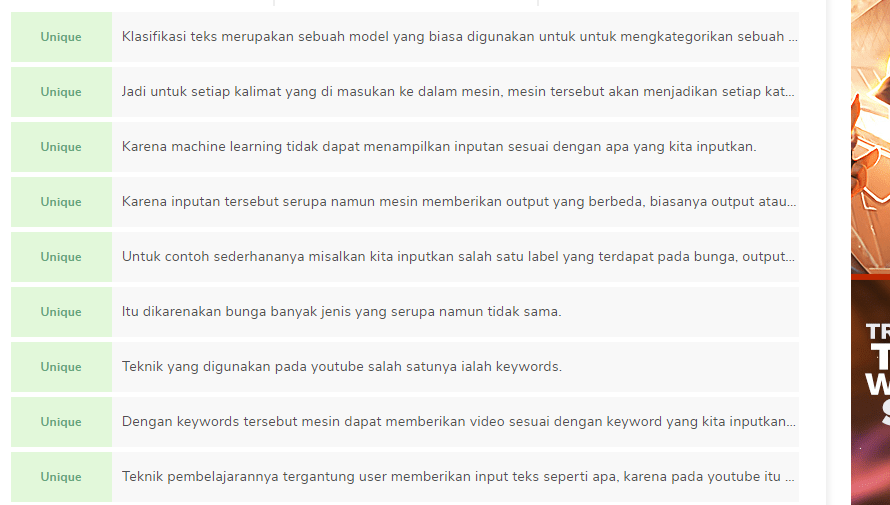
\includegraphics[width=4cm]{figures/1174095/tugas4/plag.PNG}
	\caption{Bukti Tidak Melakukan Plagiat Chapter 4}
\end{figure}
